\documentclass{beamer}
\usepackage[utf8]{inputenc}
\usepackage[spanish]{babel}
\usepackage{hyperref}
\usepackage{verbatim}
\usepackage{listings}
\usepackage{tikz}
\usetikzlibrary{arrows}

\setbeamercovered{invisible}
\usetheme{Frankfurt}
\usefonttheme{serif}

% Configurar los listings (Códigos)
\renewcommand{\lstlistingname}{Código}
\lstset{
	language=C++,               % Lenguaje
	basicstyle=\ttfamily\footnotesize,  % Tipo de fuente
	keywordstyle=\color{blue},  % Color de palabras clave
	stringstyle=\color{red},    % Color de strings
	commentstyle=\color{gray},  % Color de comentarios
	showstringspaces=false,     % No muestrar el _ cuando el string tiene espacios
	breaklines = true,          % Partir las líneas largas
	breakatwhitespace=true,	    % Partir las líneas en un espacio
	numbers=left,				% Numerar las líneas a la izq
	numberstyle=\tiny,			% Poner los números de las líneas pequeños
	numberblanklines=true,      % Numerar las líneas en blanco
	columns=fullflexible,       % No perder el formato al dejar los espacios
	keepspaces=true,   			% Dejar los espacios insertados
	frame=tb,					% Poner el recuadro
}

\AtBeginSection[]{%
  \begin{frame}<beamer>
    \frametitle{Contenido}
    \tableofcontents[sectionstyle=show/hide,subsectionstyle=hide/show/hide]
  \end{frame}
  \addtocounter{framenumber}{-1}% If you don't want them to affect the slide number
}

\title{Semillero de Programación}
\subtitle{Algoritmo de Knuth-Morris-Pratt}
\author{Ana Echavarría \and Juan Francisco Cardona}

\institute{Universidad EAFIT}
\date{26 de abril de 2013}

\begin{document}

\begin{frame}
	\titlepage
\end{frame}

\begin{frame}
	\frametitle{Contenido}
	\tableofcontents
\end{frame}

\section{Problemas semana anterior}
	\subsection{Problema A - Numbering Roads}
	
	\begin{frame}
		\frametitle{Problema A - Numbering Roads}
		\begin{itemize}
			\item Hay que representar $r$ calles con $n$ números y 26 letras
			\item El número de calles que se tienen que representar con letras son $f = r - n$
			\item El número mínimo de letras que hay que usar es $\left\lceil \frac{f}{n} \right\rceil$
			\item Si ese número es mayor que las 26 letras disponibles, es imposible.
		\end{itemize}
	\end{frame}
	
	\begin{frame}[fragile]
		\frametitle{Implementación}
		\begin{lstlisting}
			int main(){
			    int roads, numbers;
			    int cases = 1;
			    while(cin >> roads >> numbers){
			        if (roads == 0 and numbers == 0) break;
			        int remaining = roads - numbers;
			        int ans = (remaining + numbers - 1) /  numbers;
			        if (ans <= 26){
			            printf("Case %d: %d\n", cases, ans); 
			        }else{
			            printf("Case %d: impossible\n", cases); 
			        }
			        cases++;
			    }
			    return 0;
			}
		\end{lstlisting}
	\end{frame}
	
	\subsection{Problema B - Ubiquitous Religions}
	\begin{frame}
		\frametitle{Problema B - Ubiquitous Religions}
		\begin{itemize}
			\item Utilizar Union-Find para representar los diferentes conjuntos de religiones.
			\item Inicialmente se asume que todas las personas tienen una religión diferente.
			\item Cada que dos personas tengan la misma religión se unen los conjuntos de esas dos personas.
			\item La respuesta es contar el número de conjuntos diferentes.
		\end{itemize}
	\end{frame}
	
	\begin{frame}[fragile, allowframebreaks]
		\frametitle{Implementación}
		\begin{lstlisting}
			const int MAXN = 50005;
			int p[MAXN];
			bool seen[MAXN];

			int find(int u){
			   if (p[u] == u) return u;
			   return p[u] = find(p[u]);
			}
			void join(int u, int v){
			   p[find(u)] = find(v);
			}

			int main(){
			   int n, m;
			   int run = 1;
			   while (cin >> n >> m){
			      if (n == 0 and m == 0) break;
			      for (int i = 0; i <= n; ++i) p[i] = i;
			      for (int i = 0; i < m; ++i){
			         int u, v; cin >> u >> v;
			         join(u, v);
			      }
			
			      memset(seen, false, sizeof(seen));
			      int count = 0;
			      for (int u = 1; u <= n; ++u){
			         int parent = find(u);
			         if (!seen[parent]){
			            count++;
			            seen[parent] = true;
			         }
			      }
			      printf("Case %d: %d\n", run++, count);
			   }
			   return 0;
			}
		\end{lstlisting}
	\end{frame}
	
	\subsection{Problema C - Dark roads}
	\begin{frame}
		\frametitle{Problema C - Dark roads}
		\begin{itemize}
			\item Hay que hallar el mínimo costo de mantener iluminadas las calles de manera que haya un trayecto iluminado entre cualquier par de ciudades.
			\item Este costo corresponde con el minimum spanning tree del grafo.
			\item Utilizar el algoritmo de Prim / Kruskal.
			\item La respuesta es el dinero ahorrado, es decir el costo total menos el costo hallado por el MST.
		\end{itemize}
	\end{frame}
	
	
	\begin{frame}[fragile, allowframebreaks]
		\frametitle{Implementación}
		\begin{lstlisting}
			const int MAXN = 200005;
			typedef pair <int, int> edge;
			bool visited[MAXN];
			vector <pair <int, int> > g[MAXN]; 

			int prim(int n){
			   for (int i = 0; i <= n; ++i) visited[i] = false;
			   int total = 0;

			   priority_queue<edge, vector <edge>, greater<edge> > q;
			   q.push(edge(0, 0));
			   while (!q.empty()){
			      int u = q.top().second;
			      int w = q.top().first;
			      q.pop();
			      if (visited[u]) continue;

			      
			      visited[u] = true;
			      total += w;
			      for (int i = 0; i < g[u].size(); ++i){
			         int v = g[u][i].first;
			         int next_w = g[u][i].second;
			         if (!visited[v]){
			            q.push(edge(next_w, v));
			         }
			      }
			   }
			   return total;
			}
			int main(){
			   int n, m;
			   while (cin >> n >> m){
			      if (n == 0 and m == 0) break;

			      for (int i = 0; i <= n; ++i) g[i].clear();

			      int total_sum = 0;
			      for (int i = 0; i < m; ++i){
			         int x, y, c;
			         cin >> x >> y >> c;
			         total_sum += c;
			         g[x].push_back(make_pair(y, c));
			         g[y].push_back(make_pair(x, c));
			      }

			      cout << total_sum - prim(n) << endl;
			   }
			    return 0;
			}
		\end{lstlisting}
	\end{frame}

\section{String Matching}

	\begin{frame}
		\frametitle{String Matching Problem}
		El ``string mathching problem'' o ``needle in a haystack problem'' se define así:\\ \quad \\
		
		\textcolor{blue}{\large Entrada}\\
		Un string $T$ (llamado texto o haystack) de tamaño $n$\\ 
		Un string $P$ (llamado patrón o needle) de tamaño $m$ con $m\ \leq n$ \\ \quad \\
		\textcolor{blue}{\large Objetivo}\\
		Hallar todos los valores de $i$ con $0 \leq i \leq n - m$ para los cuales 
		$$T[i + j] = P[j] \text{\quad} \forall \,\, j \in [0, m-1]$$
		Es decir, todas las posiciones en el string $T$ donde ocurre la palabra $P$.\\
	\end{frame}
	
	\begin{frame}
		\frametitle{Algoritmo para String Matching}
		\begin{enumerate}
			\item Para $i$ desde 0 hasta $n-1$
			\item encontrado = true
			{\setlength\itemindent{15pt} \item Para $j$ desde 0 hasta $m-1$}
			{\setlength\itemindent{30pt} \item Si $T[i + j] \neq P[j]$} 
			{\setlength\itemindent{45pt} \item encontrado = false}
			{\setlength\itemindent{45pt} \item break}
			\item Si encontrado
			{\setlength\itemindent{15pt} \item imprimir i}
		\end{enumerate}
		\pause
		\begin{alertblock}{Complejidad}
			La complejidad de este algoritmo es $O(n \times m)$. ¿Será lo mejor que se puede lograr?
		\end{alertblock}
	\end{frame}
	
\section[KMP]{Algoritmo de Knuth-Morris-Pratt (KMP)}
	\begin{frame}
		\frametitle{Idea}
		\begin{itemize}
			\item En el algoritmo anterior, cuando se define que la cadena $P$ no ocurre en la posición $i$ de $T$, se vuelve a empezar la comparación en la posición $i+1$
			\item Sin embargo, este algoritmo no tiene en cuenta que si $P$ no ocurrió en la posición $i$ porque no coincidió el caracter $j$, esta información puede ser útil para evitar comparaciones innecesarias en la posición $i+1$
		\end{itemize}
	\end{frame}
	
	\begin{frame}
		\frametitle{Observación}
		Supongamos que los primeros $j$ caracteres de $P$ coincidieron con los caracteres de $T$ cuando se compara desde la posición $i$, pero que el caracter $P[j]$ no coincide con el $ T[i + j]$ esto es:\\ \quad \\
		$P[k] = T[i+k] \,\, \forall \, k \in [0 \ldots j)$ \quad y \quad $P[j] \neq T[i+j]$\\ \quad \\
		Para cada $0 < k < j$, si $T[i+k \ldots i + j - 1]$ no es un prefijo de $P$ entonces $P$ no puede ocurrir en la posición $i+k$. \\ \quad \\
		En otras palabras, no puede haber una ocurrencia de $P$ si en la posición $i+k$ si los caracteres de $T$ que ya se compararon ($i+k$ al $i+j-1$) no son un prefijo de $P$.
	\end{frame}
	
	\begin{frame}
		\frametitle{¿Cuál posición debe ser la siguiente en evaluarse?}
		\begin{itemize}
			\item Sea $P[0 \ldots j-1] = T[i \ldots i+j-1]$ \quad y \quad $P[j] \neq T[i+j]$\\ \quad \\
			\item Se puede reanudar la búsqueda en la posición $i+k$ con el $k$ más pequeño tal que $0 < k < j$ y
					$$T[i+k \ldots i+j-1] = P[k \ldots j-1] \text{ es un prefijo de } P$$
			\item Pero $P[k \ldots j-1]$ es un sufijo de $P[0 \ldots j-1]$ luego la búsqueda se reanuda en la posición $i+k$ tal que $P[k \ldots j-1]$ es el sufijo más largo de la cadena $P[0 \ldots j-1]$ que también es sufijo de la misma.
		\end{itemize}
	\end{frame}
	
	\begin{frame}
		\frametitle{Utilizando el borde}
		Definamos un borde de una cadena $s$ como la cadena más larga que es a la vez prefijo y sufijo de $s$ pero que es diferente de $s$.\\ \quad \\
		La idea que tuvieron Knuth, Morris y Pratt para evitarse comparaciones dobles fue la de calcular el borde para cada prefijo del patrón / needle y usarlo para evitar comparaciones innecesarias.
	\end{frame}
	
	\begin{frame}
		\frametitle{Computando el borde de cada prefijo}
		Para cada prefijo de la cadena \textcolor{blue}{ababaca} el borde es\\ \quad \\
		\begin{columns}[l]
			\column{0.05\textwidth}
				\textcolor{blue}{$\epsilon$}\\
				\textcolor{blue}{a}\\
				\textcolor{blue}{ab}\\
				\textcolor{blue}{aba}\\
				\textcolor{blue}{abab}\\
				\textcolor{blue}{ababa}\\
				\textcolor{blue}{ababac}\\
				\textcolor{blue}{ababaca}\\
			\column{0.8\textwidth}
				\pause$\rightarrow$ \textcolor{red}{$\epsilon$}\\
				\pause$\rightarrow$ \textcolor{red}{$\epsilon$}\\
				\pause$\rightarrow$ \textcolor{red}{$\epsilon$}\\
				\pause$\rightarrow$ \textcolor{red}{a}\\
				\pause$\rightarrow$ \textcolor{red}{ab}\\
				\pause$\rightarrow$ \textcolor{red}{aba}\\
				\pause$\rightarrow$ \textcolor{red}{$\epsilon$}\\
				\pause$\rightarrow$ \textcolor{red}{a}\\
		\end{columns}
	\end{frame}
	
	\begin{frame}
		\frametitle{Haciendo la comparación usando el borde}
		\begin{center} 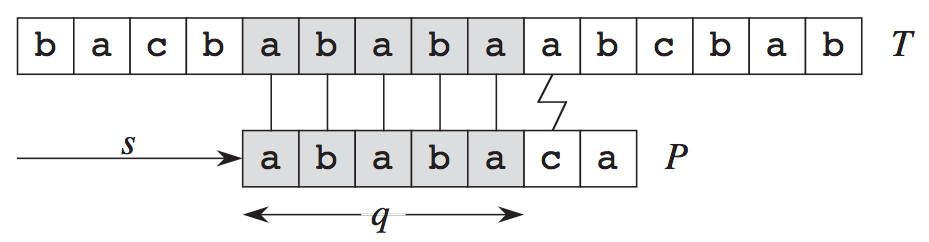
\includegraphics[height = 0.25\textheight]{Match1.png} \end{center}
		Comparando las cadenas, coincidieron los primeros 5 caracteres.\\
		El borde del prefijo de longitud 5 tiene longitud 3 por lo que la cadena se puede mover 5 - 3 = 2 posiciones a la derecha y en esa posición 3 caracteres coinciden.\\
		\begin{center} 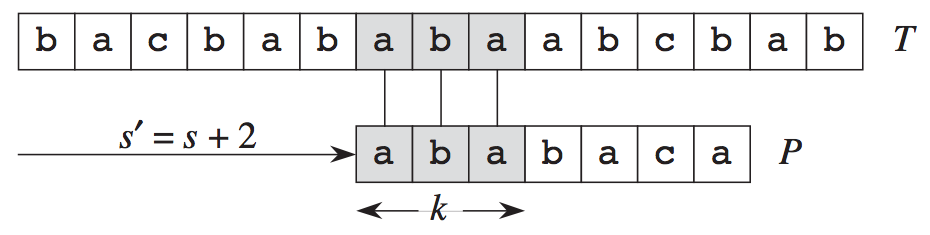
\includegraphics[height = 0.25\textheight]{Match2.png} \end{center}
	\end{frame}
	
	\begin{frame}
		\frametitle{Comparación lineal}
		Utilizando el borde de cada prefijo se puede hacer una sola comparación para cada caracter del texto T, es decir que la comparación es lineal sobre la longitud del texto.
	\end{frame}
	
	\begin{frame}[fragile]
		\frametitle{¿Cómo calcular el borde de cada prefijo?}
		Sea \verb|border[i]| la longitud del borde del prefijo de needle que termina en la posición \verb|i|.\\
		Para la cadena \textcolor{blue}{abacabacabadab}
		\begin{center}
		  \begin{tabular}{| c | c c c c c c c c c c c c c c | }
		    \hline
		    i & 0 & 1 & 2 & 3 & 4 & 5 & 6 & 7 & 8 & 9 & 10 & 11 & 12 & 13 \\ %[0.5ex]
		    \hline
		    \hline
		    \textit{needle} & a & b & a & c & a & b & a & c & a & b & a & d & a & b \\
		    \textit{border} & 0 & 0 & 1 & 0 & 1 & 2 & 3 & 4 & 5 & 6 & 7 & 0 & 1 & 2 \\
		    \hline
		  \end{tabular}
		\end{center}
		Nótese que un borde de un borde de una cadena $s$ es también un borde de $s$ por ejemplo:\\
		$s$ = abacaba, $s$ termina en la posición 6 por lo que su borde es \verb|border[6] = 3| $\rightarrow$ aba.\\
		aba termina en la posición 2 por lo que su borde es \verb|border[2] = border[border[6] - 1] = 1| $\rightarrow$ a.
	\end{frame}
	
	\begin{frame}[fragile]
		\frametitle{¿Cómo calcular el borde de cada prefijo?}
		Supongamos que se tiene calculado \verb|border[0], border[1],| $\ldots$ \verb|border[k-1]| y se quiere calcular \verb|border[k]|.\\ \quad \\
		Sabemos que \verb|P[0...border[k-1]-1]| es el prefijo más largo que también es sufijo de \verb|P[0...k-1]|. Para calcular \verb|border[k]| hay dos posibilidades:
		\begin{itemize}
			\item \verb|P[border[k-1]] = P[k]| en cuyo caso \verb|border[k] = border[k-1] + 1|.
			\item \verb|P[border[k-1]] != P[k]| se debe buscar el siguiente prefijo más grande de $P$ que también sea un sufijo \verb|P[0...k-1]|. Este prefijo tiene la longitud de border[border[k-1] - 1]| y ahora se deben comparar \verb|P[k]| con \verb|P[border[border[k-1] - 1]]|.
		\end{itemize}
		Este proceso se hace iterativamente hasta que haya una coincidencia de caracteres o hasta que se llegue a un prefijo vacío.
	\end{frame}
	
	\begin{frame}[fragile]
		\frametitle{Implementación}
		\begin{lstlisting}
			int m = needle.size();
			vector<int> border(m);
			border[0] = 0;
			 
			for (int i = 1; i < m; ++i) {
			    border[i] = border[i - 1];
			    // Mientras que el borde sea mayor que 0 y los caracteres no coincidan
			    while (border[i] > 0 and needle[i] != needle[border[i]]) {
			        border[i] = border[border[i] - 1];
			    }
			    // Si hubo coincidencia sumarle ese caracter a la longitud
			    if (needle[i] == needle[border[i]]) border[i]++;
			}
		\end{lstlisting}
	\end{frame}
	
	\begin{frame}
		\frametitle{Complejidad}
		\begin{block}{Complejidad}
			En este algoritmo se cumple (aunque no es fácil de probar) que el while interno sólo se ejecuta máximo $m-1$ veces en toda la ejecución del algoritmo.\\ \quad \\
			Es por esto que la complejidad de hallar los bordes es en total $O(m)$.
		\end{block}
	\end{frame}
	
	\begin{frame}
		\frametitle{Comparación}
		Como ya se mostró anteriormente, el arreglo de los bordes sirve para hacer la comparación rápidamente así.\\
		\begin{enumerate}
			\item Hacer seen 0 (el número de caracteres de $P$ han coincidido)
			\item Para $i$ desde 0 hasta el tamaño de $T$
			{\setlength\itemindent{15pt} \item Mientras que $seen > 0$ y $T[i] \neq P[seen]$} 
			{\setlength\itemindent{30pt} \item Comparar desde el borde de $P[0 \ldots seen-1]$, es decir $seen = border[seen-1]$}
			{\setlength\itemindent{15pt} \item Si $T[i]$ = $P[seen]$}
			{\setlength\itemindent{30pt} \item $seen = seen + 1$}
			{\setlength\itemindent{15pt} \item Si seen = tamaño de $P$}
			{\setlength\itemindent{30pt} \item Imprimir que hubo una aparición que termina en $i$}
			{\setlength\itemindent{30pt} \item $seen = seen[border[size($P$) - 1]]$}
		\end{enumerate}
	\end{frame}
	
	\begin{frame}
		\frametitle{Ejemplo}
		\begin{block}{Ejemplo}
			Utilizar el algoritmo de comparación para hallar las ocurrencias de \textcolor{blue}{\Large ababa} en el texto \textcolor{blue}{\Large bacbabababacbb}.
		\end{block}
	\end{frame}
	
	\begin{frame}[fragile]
		\frametitle{Implementación}
		\begin{lstlisting}
		int n = haystack.size();
		int seen = 0;
		for (int i = 0; i < n; ++i){
			// Buscar el borde más grande cuyo siguiente elemento sea igual al caracter que se está mirando
		    while (seen > 0 and haystack[i] != needle[seen]) {
		        seen = border[seen - 1];
		    }
		    if (haystack[i] == needle[seen]) seen++;
		    // Si en total han coincidido m = tamaño de needle caracteres, se halló la palabra
		    if (seen == m) {
		        printf("Needle occurs from %d to %d\n", i - m + 1, i);
		        seen = border[m - 1];
		    }
		}
		\end{lstlisting}
	\end{frame}

	\begin{frame}
		\frametitle{Complejidad}
		\begin{block}{Complejidad de la comparación}
			En este algoritmo se cumple que el while interno sólo se ejecuta máximo $n-1$ veces en toda la ejecución del algoritmo.\\
			Es por esto que la complejidad de hacer las comparaciones es en total $O(m)$.
		\end{block}
		
		\begin{block}{Complejidad de KMP}
			Hallar los bordes tiene una complejidad de $O(n)$ y hacer las comparaciones tiene una complejidad de $O(m)$.\\
			Como en el problema se especificó que $n \leq m$, la complejidad total de KMP es $O(n)$.
		\end{block}
	\end{frame}
	

\section{Tarea}
	\begin{frame}[fragile]
		\frametitle{Tarea}
		\begin{alertblock}{Tarea}
			Resolver los problemas de \url{http://contests.factorcomun.org/contests/58}
		\end{alertblock}
	\end{frame}

\end{document}